\documentclass{cumcmthesis}
%\documentclass[withoutpreface,bwprint]{cumcmthesis} %去掉封面与编号页。

%声明:本模板基于CUMCMThesis项目修改而来,适用于全国大学生信息安全竞赛作品赛
%仅供学习交流使用,侵删
%author:ShenaoW from XDU SCE
%cooperator:PoliScope项目组
%email:shenaowang@foxmail.com
%date:2022.05.24

\usepackage[framemethod=TikZ]{mdframed}
\usepackage{url}   % 网页链接
\usepackage{subcaption} % 子标题
\usepackage{colortbl}
\usepackage{color}
\definecolor{tabcolor}{RGB}{42, 110, 63} % 这里就是我们怎么定义我们的表格的线宽颜色
% 伪代码
\usepackage[noend]{algpseudocode}
\usepackage{algorithmicx,algorithm}
% 页眉页脚
\usepackage{lastpage}
\usepackage{fancyhdr} % 导入fancyhdr包
\pagestyle{fancy}
% 图表、公式按章节编号
\usepackage{amsmath}
\numberwithin{equation}{section} % 公式按章节编号
\numberwithin{figure}{section} % 图按章节编号
\numberwithin{table}{section} % 表按章节编号



% 设置封面页内容
\titlename{PoliScope:安卓应用隐私政策与权限调用一致性的合规检测}
\email{shenaowang@foxmail.com}
\yearinput{2024}
\monthinput{05}
\dayinput{24}

% 页眉设置
\fancyhead[L]{}
\fancyhead[R]{}
\fancyhead[C]{\zihao{-5} PoliScope:安卓应用隐私政策与权限调用一致性的合规检测}
% 页脚设置
%\fancyfoot[L]{左页脚}
\fancyfoot[C]{\zihao{-5} 第\thepage 页 \enspace 共 \pageref{LastPage} 页} % 页码
%\fancyfoot[R]{右页脚}
\renewcommand{\headrulewidth}{0.5pt} % 页眉分隔线宽度0.5磅
%\renewcommand{\footrulewidth}{0.5pt}  % 页脚分隔线宽度0.5磅

\begin{document}
	
% 将\usepackage{ulem}宏包中的\emph{}还原为斜体
\normalem

% 生成封面页和填写说明页	
\maketitle
 
% 生成目录
\newpage
\thispagestyle{empty}
\tableofcontents
\newpage
 
%% 生成图目录
%\thispagestyle{empty}
%\listoffigures
%\newpage
%
%% 生成表目录
%\thispagestyle{empty}
%\listoftables
%\newpage

% 从此处开始编页
\setcounter{page}{1}
 
%中文摘要
\begin{cnabstract}
	
(请简要说明创作本作品之动机、功能、特性、创新处、实用性)

在当今数字化时代,随着信息技术的迅猛发展,患者就诊时医疗数据的产生和积累呈指数级增长,涵盖了个人诊疗状况、疾病诊断信息和基因组数据等,这些数据在就诊时的及时传递与共享对于患者的治疗决策、疾病确诊、临床治疗等方面具有重要意义。

然而,医疗数据的安全共享和利用同样面临着极大的挑战。一方面,现有的医疗机构存储的医疗数据往往仅在内部管理共享,彼此间并不相通,造成严重数据孤岛现象,使患者在进行跨机构就诊时需要准备多份电子病历;另一方面,医疗数据中包含患者的个人隐私敏感信息,在内部共享环境下仍存在部分医疗机构内部人员在未经患者同意的情况下使用这些数据,可能会导致患者隐私泄露;此外,医疗数据还具有一定的商业价值,如利用这些数据来定向投送医疗广告等,很容易成为不法分子恶意攻击进行牟利的对象。因此,在实现医疗数据多机构共享平台的同时,能够保障个人隐私安全具有重要的现实意义。

针对这些问题,基于分布式身份(Decentralized Identifiers,DID)技术实现医疗数据共享平台的想法应运而生。DID技术基于区块链和分布式账本等技术,具有区块链透明、可追溯、不可篡改等优良特性,为每个参与者提供了独一无二的身份标识,实现了去中心化、安全、可验证的身份认证和授权管理。

通过基于DID技术的医疗数据共享平台,医疗数据的共享变得更加安全、高效和透明。医疗机构、医生、患者和研究人员可以在平台上自主管理和控制自己的数据,授权合适的权限给其他参与者,实现了医疗数据的可信共享和跨组织的协同合作。此外,基于智能合约的数据访问控制机制结合加密技术可以确保数据的安全性和隐私保护,有效解决了医疗数据共享中的信任和隐私问题。

在这样一个背景下,本文将设计与实现基于DID技术的医疗数据共享平台,分析其在促进医疗数据共享、优化医疗资源配置、保障隐私安全等方面的作用和价值,为医疗行业的数字化和个人隐私的安全保护提供支持。

(还会调整)
	
\cnkeywords{1 \quad 2 \quad 3 \quad 4}
\end{cnabstract}

%英文摘要
\begin{enabstract}


\enkeywords{Privacy Compliance \quad NER \quad Static Analysis \quad Dynamic Analysis}
\end{enabstract}

\section{作品概述}

(建议包括:背景分析、相关工作、特色描述及应用前景分析等) 

\subsection{背景分析}

在当今数字化时代,随着信息技术的迅猛发展,患者就诊时医疗数据的产生和积累呈指数级增长,涵盖了个人诊疗状况、疾病诊断信息和基因组数据等,这些数据在就诊时的及时传递与共享对于患者的治疗决策、疾病确诊、临床治疗等方面具有重要意义。

然而,医疗数据的安全共享和利用同样面临着极大的挑战。一方面,现有的医疗机构存储的医疗数据往往仅在内部管理共享,彼此间并不相通,造成严重数据孤岛现象,使患者在进行跨机构就诊时需要准备多份电子病历;另一方面,医疗数据中包含患者的个人隐私敏感信息,在内部共享环境下仍存在部分医疗机构内部人员在未经患者同意的情况下使用这些数据,可能会导致患者隐私泄露;此外,医疗数据还具有一定的商业价值,如利用这些数据来定向投送医疗广告等,很容易成为不法分子恶意攻击进行牟利的对象。可见,在实现医疗数据多机构共享平台的同时,如何保障个人隐私安全成为了医疗行业数字化的一大难题。

现有的医疗数据共享方式一般可分为两类:一种是集中式存储的医疗数据共享方式,另一种是分布式存储的医疗数据共享方式。前者使用广泛,但随时代发展暴露出如数据孤岛等诸多弊端;后者则则多以区块链技术为依托,以其分布式、匿名性、公开性和不可窜改的特点,在解决医疗信息共享问题上具有显著优势,但仍然具有xxx、xxx和xxx的弊端。因此,研究一种既能发挥分布式优势,又能减少/克服xxx、xxx的医疗数据共享方法具有重要的现实意义。

\subsection{相关工作}

\subsubsection{Weidentity区块链技术}

\subsubsection{分布式身份技术}

\subsection{特色描述}

用户可以使用其DID作为身份标识,在不同医疗机构之间共享医疗数据,如病历、检查报告、影像数据等。用户可以通过授权方式,选择性地分享特定的数据给特定的医疗机构或医生,从而避免在不同医院之间重复进行相同的检查和检验。

通过数字身份(DID)技术,我们可以实现可靠的身份验证、精细的数据共享控制、隐私保护和便捷的健康管理,从而改善医患关系。患者可以更加信任地分享健康数据,医生可以更有效地提供个性化的医疗服务,促进医疗系统的协作和效率提升。用户选择性向医生揭秘一部分数据,医生能确保这些数据是来源正确可靠的,用户不能随意伪造数据,用户也能控制数据的披露程度

\subsection{应用前景分析}

\newpage

\section{作品设计与实现}

(建议包括系统方案、实现原理、硬件框图、软件流程、功能、指标等)

\begin{table}[htbp]\zihao{5}
%\begin{table}[htbp]\small
	\centering
	\caption{一个简单的表格示例}
	%	\arrayrulecolor{tabcolor}
	\begin{tabular}{cccc}
		\toprule[1pt]
		\toprule[1pt]
		\textbf{实体标签} & \textbf{实体名称} & \textbf{实体举例} & \textbf{实体描述}\\
		\midrule
		\midrule
		CALENDAR & 日历权限组 & 设备日历信息、读取日历 & 读/写/访问日历等权限 \\
		\hline
		CAMERA & 相机权限组 & 拍摄照片、访问摄像头 & 调用相机相关权限 \\	
		\hline
		CONTACTS & 联系人权限组 & 查看通讯录、账户列表 & 读/写通讯录、账户列表等 \\
		\hline
		LOCATION & 位置权限组 & 定位服务、基站定位 & 获取粗略/精确位置等权限 \\
		\hline
		MICROPHONE & 麦克风权限组 & 录音,设备麦克风 & 访问麦克风及音频录制等权限 \\
		\hline
		PHONE & 手机状态权限组 & IDFA、SIM卡序列号 & 获取设备状态、通话记录等 \\
		\hline
		SENSORS & 传感器权限组 & 步数统计、运动与健康 & 访问设备传感器相关权限 \\
		\hline
		SMS & 短信权限组 & 短信授权、发送短信 & 读/写短信相关权限 \\
		\hline
		STORAGE & 存储权限组 & 访问相册、外部存储 & 读/写存储空间相关权限 \\
		\bottomrule[1pt]
		\bottomrule[1pt]
	\end{tabular}
	\label{tab:实体标签}%
\end{table}%

\begin{figure}[h]
	\centering
	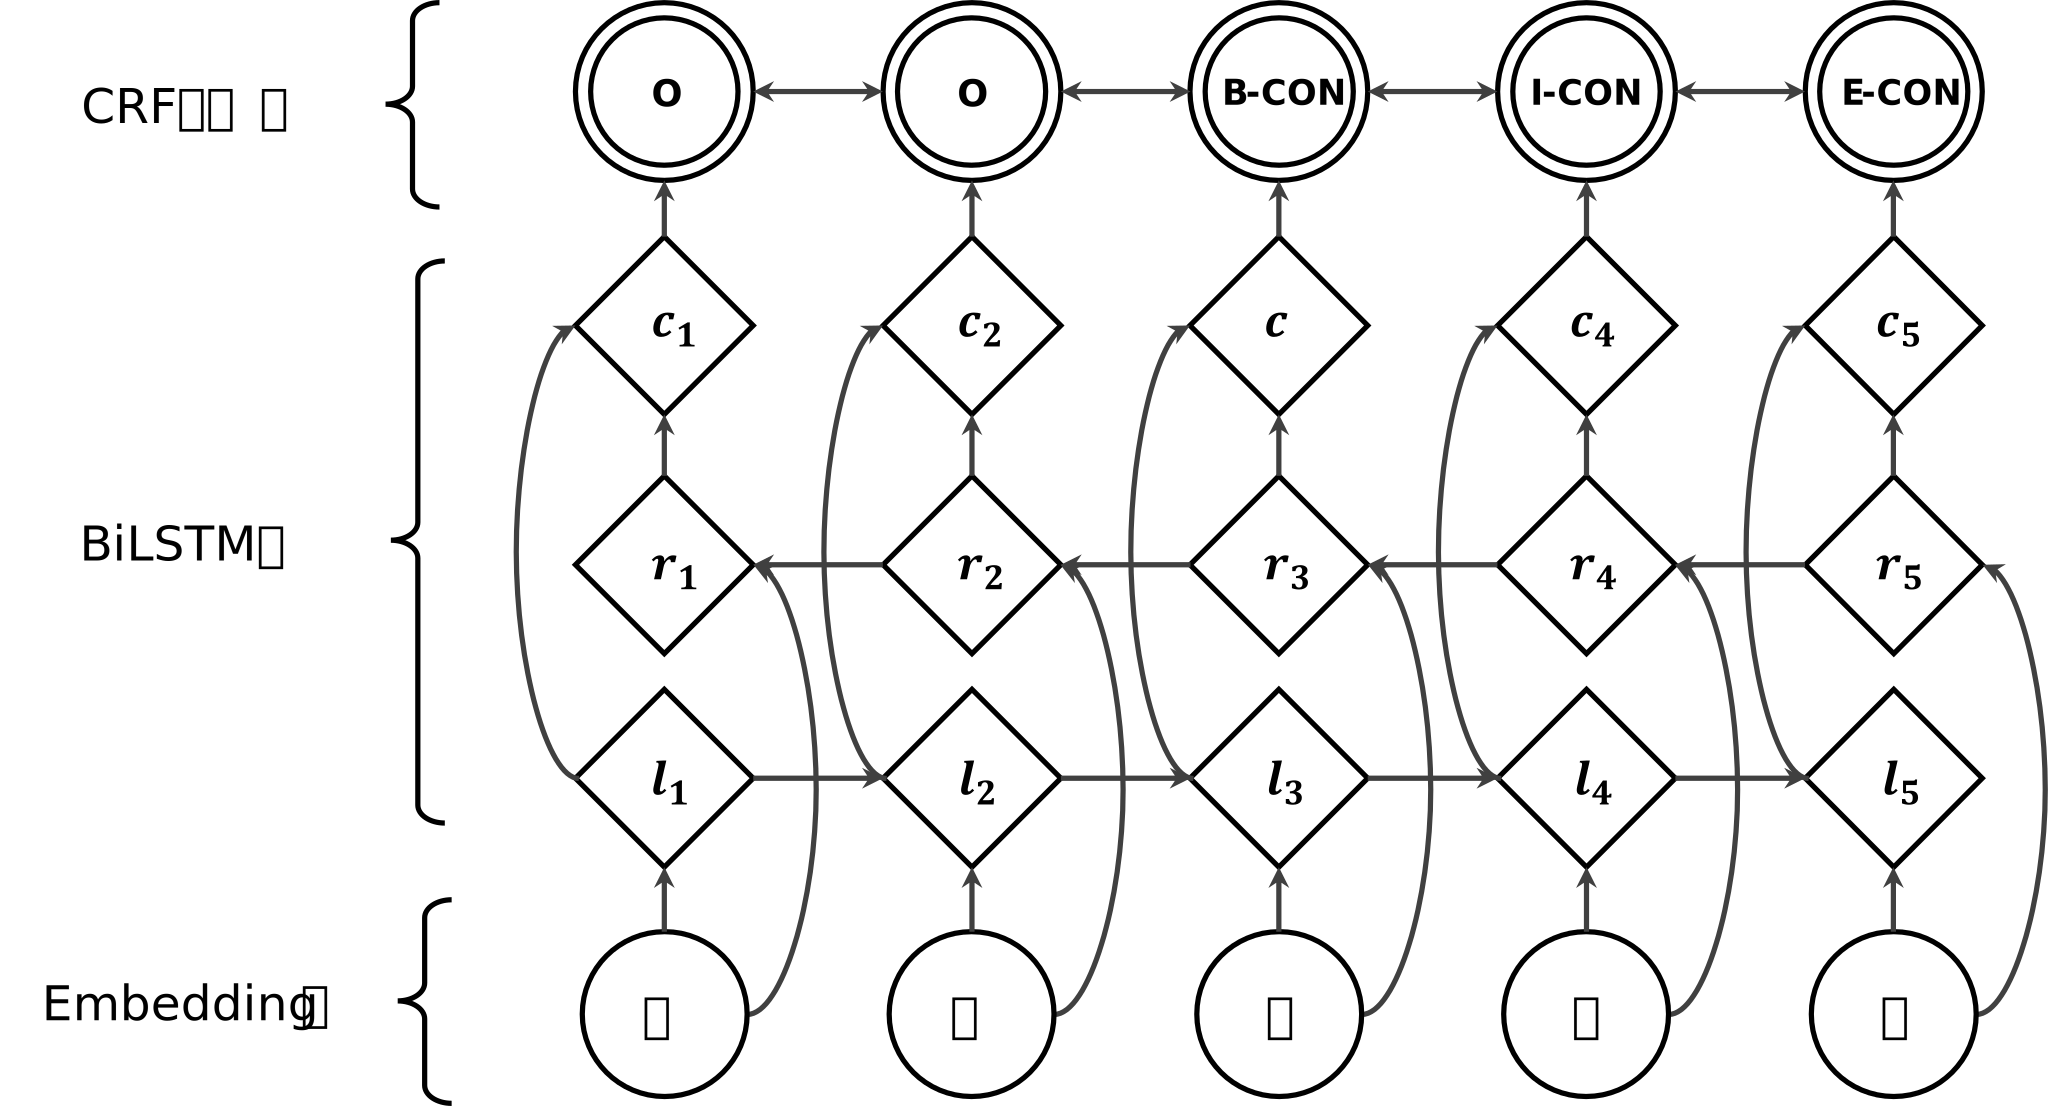
\includegraphics[width=0.85\linewidth]{ BiLSTM-CRF }
	\caption{ 图片示例 }
	\label{fig:BiLSTM-CRF}
\end{figure}

\newpage

\section{作品测试与分析}

(建议包括测试方案、测试环境搭建、测试设备、测试数据、结果分析等)


\newpage

\section{创新性说明}

(本部分内容主要说明作品的创新性)

\newpage

\section{总结}

\newpage

%参考文献
\begin{thebibliography}{9}%宽度9
	\setlength{\itemsep}{-1mm}  %% 表示参考文献间距为行间距
	
	\bibitem{工信部}工业和信息化部. 互联网和相关服务业运行情况 [EB/OL]. [2022-04-29]. https://www.miit.gov.cn/gxsj/tjfx/hlw/index.html.
    \bibitem{中消协}中国消费者协会. 100款App个人信息收集与隐私政策测评报告 [EB/OL]. [2018-11-28]. https://cca.cn/jmxf/detail/28310.html.
    \bibitem{FlowDroid}Arzt S, Rasthofer S, Fritz C, et al. Flowdroid: Precise context, flow, field, object-sensitive and lifecycle-aware taint analysis for android apps[J]. Acm Sigplan Notices, 2014, 49(6): 259-269.
\end{thebibliography}

\newpage
%附录
%\begin{appendices}
%
%\section{模板所用的宏包}
%\begin{table}[htbp]
%    \centering
%    \caption{宏包罗列}
%    \begin{tabular}{ccccc}
%        \toprule
%        \multicolumn{5}{c}{模板中已经加载的宏包} \\
%        \midrule
%        amsbsy & amsfonts & {amsgen} & {amsmath} & {amsopn} \\
%        amssymb & amstext & {appendix} & {array} & {atbegshi} \\
%        atveryend & auxhook & {bigdelim} & {bigintcalc} & {bigstrut} \\
%        bitset & bm    & {booktabs} & {calc} & {caption} \\
%        caption3 & CJKfntef & {cprotect} & {ctex} & {ctexhook} \\
%        ctexpatch & enumitem & {etexcmds} & {etoolbox} & {everysel} \\
%        expl3 & fix-cm & {fontenc} & {fontspec} & {fontspec-xetex} \\
%        geometry & gettitlestring & {graphics} & {graphicx} & {hobsub} \\
%        hobsub-generic & hobsub-hyperref & {hopatch} & {hxetex} & {hycolor} \\
%        hyperref & ifluatex & {ifpdf} & {ifthen} & {ifvtex} \\
%        ifxetex & indentfirst & {infwarerr} & {intcalc} & {keyval} \\
%        kvdefinekeys & kvoptions & {kvsetkeys} & {l3keys2e} & {letltxmacro} \\
%        listings & longtable & {lstmisc} & {ltcaption} & {ltxcmds} \\
%        multirow & nameref & {pdfescape} & {pdftexcmds} & {refcount} \\
%        rerunfilecheck & stringenc & {suffix} & {titletoc} & {tocloft} \\
%        trig  & ulem  & {uniquecounter} & {url} & {xcolor} \\
%        xcolor-patch & xeCJK & {xeCJKfntef} & {xeCJK-listings} & {xparse} \\
%        xtemplate & zhnumber &       &       &  \\
%        \bottomrule
%    \end{tabular}%
%    \label{tab:addlabel}%
%\end{table}%
%
%以上宏包都已经加载过了,不要重复加载它们。
%
%\section{排队算法--matlab 源程序}
%
%\begin{lstlisting}[language=matlab]
%kk=2;[mdd,ndd]=size(dd);
%while ~isempty(V)
%[tmpd,j]=min(W(i,V));tmpj=V(j);
%for k=2:ndd
%[tmp1,jj]=min(dd(1,k)+W(dd(2,k),V));
%tmp2=V(jj);tt(k-1,:)=[tmp1,tmp2,jj];
%end
%tmp=[tmpd,tmpj,j;tt];[tmp3,tmp4]=min(tmp(:,1));
%if tmp3==tmpd, ss(1:2,kk)=[i;tmp(tmp4,2)];
%else,tmp5=find(ss(:,tmp4)~=0);tmp6=length(tmp5);
%if dd(2,tmp4)==ss(tmp6,tmp4)
%ss(1:tmp6+1,kk)=[ss(tmp5,tmp4);tmp(tmp4,2)];
%else, ss(1:3,kk)=[i;dd(2,tmp4);tmp(tmp4,2)];
%end;end
%dd=[dd,[tmp3;tmp(tmp4,2)]];V(tmp(tmp4,3))=[];
%[mdd,ndd]=size(dd);kk=kk+1;
%end; S=ss; D=dd(1,:);
% \end{lstlisting}
%
% \section{规划解决程序--lingo源代码}
%
%\begin{lstlisting}[language=c]
%kk=2;
%[mdd,ndd]=size(dd);
%while ~isempty(V)
%    [tmpd,j]=min(W(i,V));tmpj=V(j);
%for k=2:ndd
%    [tmp1,jj]=min(dd(1,k)+W(dd(2,k),V));
%    tmp2=V(jj);tt(k-1,:)=[tmp1,tmp2,jj];
%end
%    tmp=[tmpd,tmpj,j;tt];[tmp3,tmp4]=min(tmp(:,1));
%if tmp3==tmpd, ss(1:2,kk)=[i;tmp(tmp4,2)];
%else,tmp5=find(ss(:,tmp4)~=0);tmp6=length(tmp5);
%if dd(2,tmp4)==ss(tmp6,tmp4)
%    ss(1:tmp6+1,kk)=[ss(tmp5,tmp4);tmp(tmp4,2)];
%else, ss(1:3,kk)=[i;dd(2,tmp4);tmp(tmp4,2)];
%end;
%end
%    dd=[dd,[tmp3;tmp(tmp4,2)]];V(tmp(tmp4,3))=[];
%    [mdd,ndd]=size(dd);
%    kk=kk+1;
%end;
%S=ss;
%D=dd(1,:);
% \end{lstlisting}
%\end{appendices}

%算法模板
%\begin{algorithm}[t]
%	\caption{algorithm caption} %算法的名字
%	\hspace*{0.02in} {\bf Input:} %算法的输入, \hspace*{0.02in}用来控制位置,同时利用 \\ 进行换行
%	input parameters A, B, C\\
%	\hspace*{0.02in} {\bf Output:} %算法的结果输出
%	output result
%	\begin{algorithmic}[1]
	%		\State some description % \State 后写一般语句
	%		\For{condition} % For 语句,需要和EndFor对应
	%		\If{condition} % If 语句,需要和EndIf对应
	%		\Else
	%		\EndIf
	%		\EndFor
	%		\While{condition} % While语句,需要和EndWhile对应
	%		a += 1
	%		\EndWhile
	%		\State\Return result
	%	\end{algorithmic}
%\end{algorithm}

%代码块模板
%\begin{lstlisting}[language=python]
%app_tuple_list = []
%try:
%browser.get(url)
%soup = BeautifulSoup(browser.page_source, features='lxml')
%except requests.HTTPError:
%return "There are some errors when get the download page!"
%all_app_tag = soup.find('ul', {"class": "applist", "id": "all-applist"})
%app_tag = all_app_tag.next
%\end{lstlisting}

\end{document} 